\documentclass[twoside]{article}
\usepackage{aistats/aistats2022}
% If your paper is accepted, change the options for the package
% aistats2022 as follows:
%\usepackage[accepted]{aistats2022}

% If you set papersize explicitly, activate the following three lines:
%\special{papersize = 8.5in, 11in}
%\setlength{\pdfpageheight}{11in}
%\setlength{\pdfpagewidth}{8.5in}

\let\oldsection\section
\renewcommand{\section}[1]{\oldsection{\texorpdfstring{\uppercase{#1}}{#1}}}

% If you use natbib package, activate the following three lines:
\usepackage[round]{natbib}
\renewcommand{\bibname}{References}
\renewcommand{\bibsection}{\subsubsection*{\bibname}}

\usepackage[utf8]{inputenc} % allow utf-8 input
\usepackage[T1]{fontenc}    % use 8-bit T1 fonts
\usepackage{hyperref}       % hyperlinks
\usepackage{url}            % simple URL typesetting
\usepackage{booktabs}       % professional-quality tables
\usepackage{microtype}      % microtypography
\usepackage{graphicx}
\graphicspath{{figs/}}
%\usepackage{subfigure}
\usepackage{subcaption}
\usepackage{placeins}
\usepackage{hyperref}       % hyperlinks
\usepackage[dvipsnames]{xcolor}

\usepackage{array}

\hypersetup{ % SLJ: my standard paper setup...
	pdftitle={MAP convergence},
	pdfkeywords={},
	pdfborder=0 0 0,
	pdfpagemode=UseNone,
	colorlinks=true,
	linkcolor=blue, %mydarkblue,
	citecolor=blue, %mydarkblue,
	filecolor=blue, %mydarkblue,
	urlcolor=blue, %mydarkblue,
	pdfview=FitH,
	pdfauthor={Anonymous},
}

\usepackage[capitalise]{cleveref}
\newcommand{\rlp}[1]{\textcolor{BrickRed}{(RLP:#1)}}
\newcommand{\fdk}[1]{\textcolor{Periwinkle}{(fdk:#1)}}
\newcommand{\TODO}[1]{\textcolor{cyan}{(TODO #1)}}
\newcommand{\tocite}{\textcolor{purple}{(add citation)}}

% my packages
\usepackage{math_commands}
% some custom math commands
\newtheorem{proposition}{Proposition}
\newcommand*{\expect}[2][]{\ensuremath{\mathbb{E}_{#1} \left[ #2 \right] }} % expectation operator
\newcommand*{\expecti}[2][]{\ensuremath{\mathbb{E}_{#1} [ #2 ] }} % expectation operator

\newcommand{\cond}{\,\vert\,}
\newcommand{\logpart}{A}
\newcommand{\conj}{\logpart^*}
\newcommand{\bregman}{\cB_\logpart}
\newcommand{\bregmanconj}{\cB_{\logpart^*}}
\newcommand{\nat}{\theta}
\newcommand{\m}{m}
\newcommand{\meanp}{\m}
\newcommand{\decrement}{D}
\newcommand{\linear}{\ell} % linearization of a function
\newcommand{\lr}{\gamma} % learning rate, or step-size
\newcommand{\lin}[1]{\left\langle#1\right\rangle}

\newcommand{\MAPm}{\hat \m_n}
\newcommand{\MAPt}{\hat \nat_n}
\DeclareMathSymbol{\shortminus}{\mathbin}{AMSa}{"39}


%\hypersetup{draft}

\begin{document}

% If your paper is accepted and the title of your paper is very long,
% the style will print as headings an error message. Use the following
% command to supply a shorter title of your paper so that it can be
% used as headings.
%
%\runningtitle{I use this title instead because the last one was very long}

% If your paper is accepted and the number of authors is large, the
% style will print as headings an error message. Use the following
% command to supply a shorter version of the authors names so that
% they can be used as headings (for example, use only the surnames)
%
%\runningauthor{Surname 1, Surname 2, Surname 3, ...., Surname n}

\twocolumn[

\aistatstitle{Convergence Rates for the MAP of an Exponential Family, and Stochastic Mirror Descent -- an Open Problem}


\aistatsauthor{R\'emi Le Priol \And Frederik Kunstner \And  Damien Scieur \And Simon Lacoste-Julien }

\aistatsaddress{ Mila \And  UBC \And SAIT SAIL \And Mila}
]

\begin{abstract}
We consider the problem of upper bounding the expected sub-optimality of the maximum likelihood estimate (MLE), or a conjugate maximum a posteriori (MAP) for an exponential family.
Surprisingly, we found no general solution to this problem in the literature.
In particular, current theories do not hold for a Gaussian, or in the very interesting few samples regime.
After exhibiting various facets of the problem, we show the MAP can be interpreted as the result of Stochastic Mirror Descent (SMD),
yet it falls out of scope for modern analysis.
We believe solving this very fundamental problem may bring progress to both the statistics and optimization communities.
\end{abstract}

%In particular, no rates hold in the few samples regime  -- e.g. after seeing 5 samples from a gaussian, we do not know how many bits away from the true distribution we should expect our model to be.
%No rates hold either when the loss is ill-behaved : infinite domain, not smooth, not self-concordant


\begin{figure}[t]
	\centering
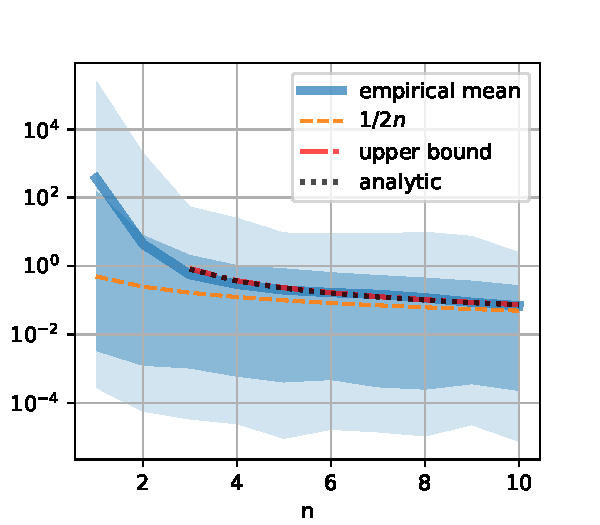
\includegraphics[width=.4\textwidth]{fewsamples.pdf}
	\caption{Suboptimality of a Gaussian variance MLE against number of samples $n$. Bold curve is average over 100 trials,  dark shaded area is 90\% (dark) confidence interval, light shade is min-max interval.
		While the expected value is infinite for $n=1$ or $n=2$, it quickly matches the upper bound, and the $1/2n$ asymptote.
	}
	\label{fig:curves}
\end{figure}


\section{Motivation}

We kind of know how to do optimization
on smooth, strongly convex functions
when there is some bound on the stochasticity,
for example in the form of a bounded variance,
say for the problem
\begin{equation} %We might want to add a feasible set for theta?
\min_\theta f(\theta)
\end{equation}
with access to stochastic gradients
$g(\theta)$ such that
\begin{equation}
	\expect{\norm{g(\theta) - \nabla f(\theta)}^2} \leq \sigma^2.
\end{equation}
Estimating the mean of Gaussian noise is a special case of this problem class, using
$f(\theta) = \frac{1}{2}\norm{\theta - \mu}^2$ and $g(\theta) \sim \cN(- \mu, \sigma^2)$.
SGD with a decreasing step-size coincides with the maximum likelihood estimate (MLE),
and attains the $1/t$ convergence rate.

But our understanding of stochastic optimization lacks in other domains.
A generalization of the above problem, at the intersection of optimization and statistics,
is the problem of minimizing
\begin{equation}
	f(\theta) = \expect[x \sim p(x\cond\theta_*)]{-\log p(x\cond\theta)},
\end{equation}
When $p(x\cond\theta)$ is an exponential family distribution,
$-\log p(x\cond\theta) = A(\theta) - \lin{t(x), \theta}$ (omitting the reference distribution).
Here, $A$ is the log-partition function, a Legendre function that we assume can be minimized in closed form.
The Gaussian example is the special case $A(\theta) = \frac{1}{2}\norm{\theta}^2$.

Typical works on parameter estimation bound the deviation with norms -- e.g. bounding $\expect[p(x\cond\theta_*)]{\norm{\theta-\theta_*}^p}$ for some norm and some power. \tocite
Or more generally, they  use distances rather than divergences as they are symmetric and usually behave smoothly. \tocite 
A contrario the KL is not smooth, and it can be infinite in misspecified settings.
But as the MLE is the minimizer of the log-likelihood, we wish to bound the sub-optimality.


There are algorithms for this setting, for example the MLE -- the (online) maximum likelihood after seeing $t$ samples -- or adding regularization, the MAP -- the maximum a posteriori. As we show, the MAP can be interpreted as online mirror descent with decreasing step-sizes. Despite recent advances in this field, our convergence rates are still lacking; they are either asymptotic, cover only special cases or require having seen many ($n \gg d$) samples.

Other works focus instead on the online estimation of $\theta$ and minimize the \textit{regret}
\[
R_T=\sum_{t=1}^T f_t(\hat{\theta}_t)-\min_{\theta\in\Theta}\sum_{t=1}^Tf_t(\theta),
\]
where $f_t(\theta)\triangleq-\log p(x_t|\theta)$, and the estimator $\hat{\theta}_t$ is computed using only the $t-1$ samples $\{x_i\}$. Usually, the \textit{follow-the-leader} strategy works best, i.e., moving the current estimate towards $x_i$ with a certain step size schedule. Unfortunately however, their rate are worse than the offline MAP or MLE algorithms. For instance, in the specific case where we estimate the mean parameter of a Bernoulli or Gaussian distribution, \citet{azoury2001relative} show that $R_T\leq log(T)$. From this bound, we can deduce the rate  to the real mean parameter, being $f(\hat{\theta}_T)-f^*\leq \frac{log(T)}{T}$. Also, \citet{dasgupta2007online} proves the asymptotic rate $\lim\sup_{T>1}\frac{R_T}{T}\leq 0$ when we estimate the mean and variance of a Gaussian, under the (strong) assumption that the data are finite, i.e., $\|x_t\|<C$. This means the estimator converges asymptotically, but with an unknown rate of convergence, therefore highlighting the difficulty of that setting.


We do not have a solution. The goal of this paper
is to bring this issue to the attention of the community working at the intersection of machine learning, optimization and statistics,
in the hope that we can make progress on this question;
Can we build algorithms for stochastic estimation
when the objective function is not (close to) quadratic
and the noise is not Gaussian?

We are aware that \emph{a} solution to this problem would be the maximum likelihood estimate for which there is a wealth of asymptotic and large sample results \citep{van2000asymptotic,ostrovskii2021finite}. %TODO complete
However, none of the theory we found could address for instance the case of a Gaussian with unknown mean and variance $\cN(\mu,\sigma^2)$, hence our contributions.
%TODO kind of redundant "problem - question - problem" paragraphs, not disentangling stats and optim. To improve

\paragraph{Contributions}
\begin{itemize}
	\item We provide insights on different facets of this problem : quadratic approximations ; bias variance decomposition; and a detailed analysis of the Gaussian variance estimation problem.
	\item We show the connections between the optimization and statistical estimation view of the problem and discuss where current theories fail to fully capture the problem.
\end{itemize}

The statistics and optimization perspective are so tightly linked in this problem, that we believe progress from one field would help the other one.
Progress from statistics could bring forward research in non-euclidean optimization, or the optimization of barrier losses, for instance helping in the development of accelerated methods.
On the other hand, optimization can become  a more versatile and general tool for statisticians. % handwavy and shady af.


% Then;
% - description of the setting
% - statistical solutions (asymptotic, l1 or l2 error)
% - optimization solutions (online+bounded gradient, self-concordance, more recent relative smoothness results)
% - potential application of ideas that would solve this, beyond this problem (acceleration, causality?)
% - conclusion?

\paragraph{Notation}
$\langle \cdot , \cdot \rangle$ is the Euclidean scalar product in $\real^d$.

\section{Technical background}

Exponential families are to statistics what linear models are to regression.
Many classical model are exponential families, for instance the Gaussian or Bernoulli distributions. Their convexity or modeling flexibility make them one of the most widely used statistical models. In this section, we review some of their properties.
We point the reader towards \citet[Chapter 3]{wainwright2008graphical} for a full review.


The exponential family for data $X\in \cX$ reads
\begin{equation}
	 p(X|\nat) = \exp( \langle \nat, T(X) \rangle - \logpart(\nat)) \; ,
	 \label{eq:def_expfamily}
\end{equation}
where  $\nat$ is called natural (or primal) parameter is specified by 1) $T: \cX \rightarrow \real^d$, the sufficient statistic, and 2) $\nu(dx)$, the density with respect to a base measure.
The function $\logpart$ is called the log-partition function that acts as a normalization term, since
\begin{align}
    \logpart(\nat) = \log \int e^{\langle \nat, T(x) \rangle} \nu(dx) \; .
\end{align}

This simple model encompasses both categorical distributions : $\cX = \{1, \dots, k\}$, $\nu$ uniform and $T(X)$  the one-hot encoding, and multivariate normal distributions $\cX=\real, \nu$ Lebesgues and $T(X)=(X, X^2)$.

For convenience, in this paper we focus on steep, regular exponential families
where $\logpart$ is strictly convex function of Legendre type,
and the set $\nat \in \Theta$ such that $\logpart(\nat) < \infty$ is open and convex
(See \citet{barndoffnielsen2014information}). Also, when explicit, we write the random variable $T = T(X)$.

% TODO sort out relationships between : steep family, minimal statistics and Legendre type. What implies what ?

\paragraph{Duality}
The logpartition function $\logpart$ verifies the two following identities:
\begin{align}
    \nabla\logpart(\nat) &=  \expect[p(T|\nat)]{T} =: \meanp \\
    \nabla^2 \logpart(\nat) &= \Cov_\nat[T] \geq 0
\end{align}
where $\meanp$ is called the mean (or dual) parameter, which lives in the open convex set $\cM$ equal to the relative interior of the convex hull of $T(\cX)$.
We will write interchangeably $\m$ or  $\nat$ depending on the context, being aware that both represent the same distribution.

We now introduce the convex conjugate (a.k.a. Fenchel-Legendre transform) of the logpartition function
\begin{align}
	\conj(\m) = \min_{\nat\in\Theta}\langle \m, \nat \rangle - \logpart(\nat) \; ,
\end{align}
which matches the common notion of \textit{entropy} in information theory. In this paper, we assume that the sufficient statistic $T$ is minimal, e.g., its covariance is definite positive for all $\nat$. In such case, the log-partition function $\logpart$ is strictly convex and its gradient $\nabla \logpart$ is a \textit{bijection} between natural parameters $\nat$ and mean parameters $\m$, and moreover, $\nabla\conj=\nabla\logpart^{-1}$ (cf Fig.~\ref{fig:duality}). More concisely,
\[
	\nabla\conj \circ \nabla\logpart(\nat) = \nat, \quad \nabla\logpart\circ \nabla\conj(\meanp) = \meanp.
\]

% The entropy is eating mean parameters, and its gradient is mapping back to natural parameters $\nabla\conj \circ \nabla\logpart(\nat) = \nat$ (cf Fig.~\ref{fig:duality}).

\begin{figure}[t] % @remi In the figure you use mu instead of m??
	\centering
	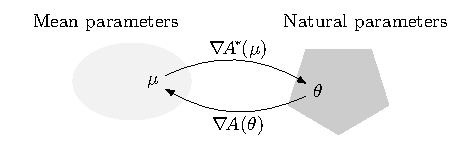
\includegraphics{duality}
	\caption{The gradient of the log-partition function and its dual, $(\nabla \logpart, \nabla \conj)$, form a bijection between natural and mean parameters $\nat, \meanp$. Figure copied from \citet{kunstner2020homeomorphic}. % TODO make an original one.
	}
	\label{fig:duality}
\end{figure}

\paragraph{Bregman Divergences} %Not super convinced about introducing that here? it comes naturally when considering the KL on exponential maps)
We now introduce the Bregman divergence induced by $\logpart$, that measure the distance between two parameters $\nat$ and $\nat_0$,
\begin{align}
    \bregman (\nat ; \nat_0)
    & = \logpart(\nat) - \logpart(\nat_0)
    - \langle \nabla \logpart(\nat_0)  , \nat - \nat_0 \rangle,
\end{align}
with $\nabla \logpart(\nat_0) = \expect[\nat_0]{T(X)} =: \meanp_0$ the mean parameter associated to $\nat_0$. In general, bregman distances are non-symmetric, i.e., $\bregman (\nat ; \nat_0)\neq \bregman (\nat_0 ; \nat)$. Finally, it is equal to the divergence of its convex conjugate with switched arguments,
\begin{align}
	\bregman (\nat ; \nat_0)
    = \bregmanconj ( \meanp_0 ; \meanp) \; .
\end{align}

\paragraph{Conjugate Prior}
One conjugate prior \citep{agarwal2010geometric} for $p(X|\nat)$ is
\begin{align}
    p(\nat)
    &\propto \exp( - n_0 \bregman(\nat ; \nat_0) ) \\
    &\propto \exp(n_0 \langle \m_0, \nat \rangle - n_0 \logpart(\nat)),
    \label{eq:def_prior}
\end{align}
where $n_0$ and $\nat_0$ are (hyper)parameters of the prior.
This is the formula for the exponential family with sufficient statistics $(\nat ,\logpart(\nat))$ and with natural parameter $(n_0 \m_0, -n_0)$.
Intuitively, $n_0$ is the number of fictive data points observed from a distribution with parameter mean $\nat_0$.

\paragraph{Maximum A Posteriori (MAP).} 
\textcolor{red}{\textbf{D.S.: This section is very unclear. }}
Using Bayes rule with~\eqref{eq:def_expfamily}~\&~\eqref{eq:def_prior}, the posterior of $\nat$ given a dataset $\mD_n =(X_1,\dots,X_n)$ is
\begin{align}
	p(\nat \cond \mD_n)
	%\propto p(\mD|\nat)p(\nat)
    \propto \exp(- (n_0+n) \bregman(\nat; \MAPt^\text{MAP}))
    \label{eq:joint_likelihood}
\end{align}
reaching its maximum in $\MAPt^\text{MAP}$ such that
\begin{align}
    \nabla \logpart(\MAPt^\text{MAP}) = \MAPm^\text{MAP}
    = \frac{n_0 \meanp_0 + \sum_{i=1}^n T_i}{n_0+n} \; .
\end{align}
where $T_i=T(X_i)$.
When $n_0=0$ -- eg we observed zero samples from the prior -- we recover the Maximum Likelihood Estimate (MLE)
\begin{align}
	\hat \m_n^\text{MLE} = \frac{\sum_{i=1}^n T_i}{n}
\end{align}
This last equation is known as moment matching.
In general, we will write $\MAPt$ to refer to the MAP, and view the MLE as a very special case.
The MLE and MAP estimates are statistics of the dataset $\mD_n$.
Given a random dataset, we wish to bound their deviation from the optimum $\nat^*$ or $\meanp^*$.


\section{Open Problem}
Given a distribution $\cD$, our objective is the expected log-likelihood 
\begin{align}
	f(\nat) = \expect[X \sim \cD]{-\log p(X \cond \nat)} 
	 = \logpart(\nat) - \langle \E[T] , \nat \rangle
\end{align}
Note that $\cD$ does not have to be part of the exponential family.
Let $\nat^* := \argmin f(\nat)$.
Assuming $\nat^*$ exists within $\Theta$ means $\cD$ is such that $\E[T] = \meanp^* \in \cM$.
Then the suboptimality on the population log-likelihood can be written with Bregman divergences
\footnote{
Since $f$ is also the KL (up to a constant)  $f(\nat) + \cst = \KL(\cD || \nat) := \KL(\cD || p(\cdot \cond \nat))$, 
and for exponential families $\bregman(\nat ; \nat^*) = KL(\nat^* || \nat)$, we recover the Pythagorean theorem of information geometry $KL(\cD || \nat) = \KL(\cD || \nat^*) + \KL(\nat^* || \nat)$.
}
\begin{align}
	 f(\nat) - f(\nat^*)
	 %&= \logpart(\nat) - \logpart(\nat^*) - \langle \E[T] , \nat - \nat^* \rangle \\
	 = \bregman(\nat ; \nat^*) 
	 = \bregmanconj(\m^* ; \m) \; .
\end{align}
Our question is: how does this suboptimality behave when $\nat$ is the MLE or the MAP ? Can we get upper-bounds in expectations ? e.g. on these quantities
\begin{align}
	\label{eq:bregmanMLE}
	\expect[\mD]{\bregmanconj \left (\E [T] ;  \inv{n}  \smallsum_i T_i \right )} \\
	\label{eq:bregmanMAP}
	\expect[\mD]{\bregmanconj \left (\E [T] ; \frac{n_0 \m_0 + \smallsum_i T_i}{n_0+n} \right )}
\end{align}
where the outer expectation is on the dataset $\mD = \{X_1, \dots, X_n \}$ sampled i.i.d from $\cD$.
More explicitly, can we write an upper bound that does not involve this expectation over the dataset.

In general, for arbitrary distributions $\cD$, it is a hard problem, especially since the KL is known for being brittle to misspecification \tocite, so let us focus on the well-specified case first $\cD = p(\cdot \cond \nat^*)$. Surely this problem has been solved, hasn't it ?
In some special cases yes, but it seems the general answer is no. 
We are yet to find a solution encompassing a broad range of exponential families, and applicable to small sample sizes $n$.

{\bf Remark.}
This could be seen as a concentration inequality, expressed with a Bregman divergence instead of a norm.
However there is a connection between the random variable $T(X)$ and the metric $\logpart$.
Indeed expressions~\eqref{eq:bregmanMLE} or~\eqref{eq:bregmanMAP} can be infinite for another choice of random variable.
For instance, if we plug in $\conj(\m)= -\log(\m)$, which defines a divergence on positive numbers, and $T(X) \sim \cN(0,1)$ which can be negative.

{\bf Remark 2.}
The expectation of the MLE may be infinite, for instance with $\cN(0,\sigma^2)$ and $n\leq 2$. Instead of taking the expectation,  we might want to bound this quantity in high probability, without resorting to Markov inequality, but that is a difficult endeavor.

\section{Insights}

\subsection{Asymptote}
As a reference point for any finite convergence rate, it is interesting to know the asymptotic behavior of these quantities as $n \rightarrow +\infty$.
Asymptotic results typically show that natural parameters $\nat$ is asymptotically normal ; reaching the Cramer-Rao lower bound \citep[for instance Ch4.2]{van2000asymptotic}.
Here the MAP is more simply expressed with mean parameters $\meanp$.
We get the asymptote by approximating the Bregman divergence using a second order Taylor expansion
\begin{align}
    \bregmanconj(\m^* ; \m)
    &= \frac{\norm{\m^* - \m}^2_{\mF^*}}{2}
    + O(\norm{\m - \m^*}^3),
\end{align}
where the Mahalanobis norm  $\| x \|_{\mF^*}^2 = x^\top \mF^* x$  is induced by $\mF^*  := \nabla^2\conj(\m^*)$, the hessian of the entropy at the optimum. It happens that  $F^*$ is also the inverse \textit{Fisher information matrix}, since
\begin{align}
    \mF^*
    :=\nabla^2\conj(\m^*)
    = \nabla^2\logpart(\nat^*)^{-1}
    = \Cov_{\nat^*}[T(X)]^{-1}  \; .
\end{align}
From there, it is possible to show an asymptotic rate for the MLE and the MAP \textcolor{red}{D.S.: How?}
\begin{align}
\label{eq:MAP_asymptote}
	\E \bregmanconj \left (\E [T(X)] ; \hat \meanp_n^\text{MLE/MAP} \right )
	= \frac{d}{2n} + O(n^{- \frac{3}{2}}) \; .
\end{align}
Both MLE and MAP have the same asymptote, as the contribution of the prior $n_0 \meanp_0$ gets negligible compared to the data for large $n$.
This asymptote is also independent of the optimum $\meanp^*$.

\subsection{Quadratic Case}
As another reference point, let us consider the case $\logpart(\nat) = \half \norm{\nat}_2^2$.
For instance, this is the log-partition of a Gaussian with variance $1$ and unknown mean 
\[ \cX=\real, \nu(dx) = \exp(\half[-x^2])dx, T(X)=X$).\]
Then $\conj(\meanp) = \half \norm{\meanp}_2^2$ as well, and both Bregman divergences are squared $\ell^2$ distances:
\begin{align}
	\bregmanconj(\meanp^* ; \meanp) = \half \norm{\meanp^* -  \meanp }_2^2  \; .
\end{align}
Thanks to the independence of samples, we can break down the MLE into individual point's contributions
\begin{align}
	\expect{\half \norm{\m^* -  \inv{n}  \smallsum_i T_i}_2^2}.
	=\frac{\Var(T)}{2n}
\end{align}
Adding a reference mean $\m_0$ to get the MAP yields to
\begin{align}
	\expect{\bregmanconj(\meanp^*; \MAPm)}
	&= \frac{n \Var(T) +  n_0^2 \norm{\m^* -  \m_0}^2}{(n+n_0)^2}.
	%\\ &= O\left(\frac{\Var(T)}{n} \right) + O\left(\frac{\norm{\m^* -  \m_0}^2}{n^2} \right)
	\label{eq:MAP_quadratic}
\end{align}
In both cases, we have a variance term in $O(n^{-1})$ and a bias term in $O(n^{-2})$. Ideally, such result should also similarly for arbitrary exponential families.
If we make restrictive assumptions on the log-partition function, we can relate $\bregmanconj$ to a norm or a quadratic.

{\bf If $\conj$ is $L$-Lipschitz} (e.g. $\logpart$ is defined within the $\ell^2$-ball of radius $L$), then
\begin{align}
    \bregmanconj(\m^* ; \m)
    &\leq L \norm{\m^* - \m} + \norm{\nat} \norm{\m^* - \m} \\
    &\leq 2L \norm{\m^* - \m}
\end{align}
so $\bregmanconj$ is $2L$-Lipschitz, and we get a $O(\inv{\sqrt{n}})$ rate.

{\bf If $\conj$ is $L$-smooth} (e.g. $\logpart$ is $\frac{1}{L}$-strongly convex), then
\begin{align}
    \bregmanconj(\m^* ; \m)
    \leq \frac{L}{2} \norm{\m^* - \m}^2
\end{align}
so $\bregmanconj$ is upper bounded by a quadratic, and we get~\eqref{eq:MAP_quadratic} as an upper bound.

\subsection{Locally Quadratic Case}
\textcolor{red}{Check this! In our case, since we assume $A$ and $A^*$ to be strictly convex,}
all Bregman divergences are locally quadratic.
Under some assumptions, like self-concordance \citep[Ch.4.1]{nesterov2003introductory}, we can quantify when this quadratic behavior kicks in.
For instance, when $T$ is 1-dimensional, we have that $\logpart$ in the following settings:
exponential distribution,
Gaussian with known mean,
Laplace with known mean,
Pareto with known minimum value,
Weibull with known shape $k$. This also holds when
-- or when $T$ lives in a compact \citep{bubeck2015entropic}. Then the bound
\begin{align}
	 \bregmanconj(\m^*,\m) \leq \norm{\m^*-\m}_{\mF^*}^2
\end{align}
holds whenever $\norm{\m^*-\m}_{\mF^*} < 0.21$.\footnote{The value of $x$ such that $x^2 \geq -\frac{x}{1-x} - \log(1 - \frac{x}{1-x})$}
Similarly, \citet{kakade2010learning} assumes a bound on all higher order moments at $\nat^*$ to quantify when $\logpart$ starts behaving quadratically, but their rate does not directly apply to $\conj$ and $\m$.

\TODO{Reference \citet{ostrovskii2021finite}.} ( as well as
\citet{anastasiou2017bounds},
\citet{marteauferey2019beyond})

All these works give \textit{large sample} results -- results that hold only for $n\geq N$ for some constant $N$ -- but none of them  apply to small $n$.

\subsection{Bias-Variance Decomposition} % DS: Arrived here
In both examples (add link), the upper bound takes the form $O(\inv{n}) + O(\frac{\text{bias}}{n^2})$, reminding us of the bias-variance decomposition. In fact, it is possible to write such a decomposition for any Bregman divergence
Let $\tilde \theta_n := \expecti{\hat \theta_n}$ be the expectation of the MAP in primal space, and $\tilde \m_n = \nabla \logpart(\tilde \theta_n )$ be the corresponding mean parameter.
As described by \citet[Theorem 0.1]{pfau2013generalized}, the  expected Bregman decomposes like
\begin{align}
	\expect{\bregmanconj(\m^* ; \hat \m_n)}
	&= {\bregmanconj(\m^* ; \tilde \m_n)}
	+ {\expect{\bregmanconj(\tilde \m_n ; \MAPm)}}
	\label{eq:primal_pivot}
\end{align}

\textbf{Remark:} In this decomposition, the primal expectation $\expect{\hat \theta_n}$ is taking the role of pivot / reference point. An estimator will be unbiased if its primal expectation is non-zero.
This is not true for the MLE. In fact for the gaussian variance MLE, the bias decreases like ${\bregmanconj(\m^* ; \tilde \m_n)} \leq \frac{2}{n(n-2)}$.
A contrario, the MLE is unbiased wrt the dual parameter, but the decomposition there is not clean.

\paragraph{Illustrations.}
We show these decompositions for $\cN(0,\sigma^2)$ in Figure~\ref{fig:variance_decomposition} and  $\cN(\mu, \sigma^2)$ in Figure~\ref{fig:gaussian_decomposition}.
In particular for $\cN(\mu, \sigma^2)$, we illustrate the characters featured in these decompositions $\hat \m_n^\text{MLE},\hat \m_n^\text{MAP},\m_n,\tilde \m_n, \m^*$ and $\m_0$ (and corresponding primal parameters)  in Figure~\ref{fig:bias-variance-numerical}. \rlp{Tune figures.}


\begin{figure}[t]
	\centering
	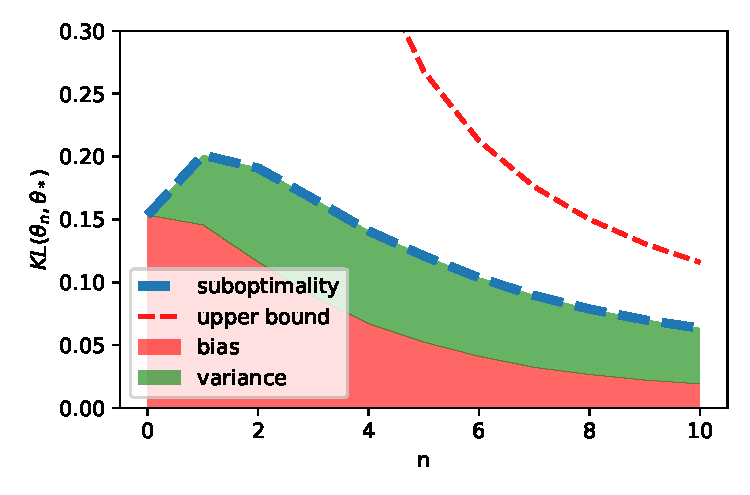
\includegraphics[width=.4\textwidth]{{figs/gaussian_variance.pdf}}
	\caption{
	\textbf{Gaussian variance $\cN(0,\sigma^2)$ example. Left:} training curves and analytic upper bound.
	\textbf{Center:} bias-mixed-variance decomposition, using the arithmetic mean.
	\textbf{Right:} bias-variance decomposition, using the harmonic mean.
	}
	\label{fig:variance_decomposition}
\end{figure}

\begin{figure}[t]
	\centering
	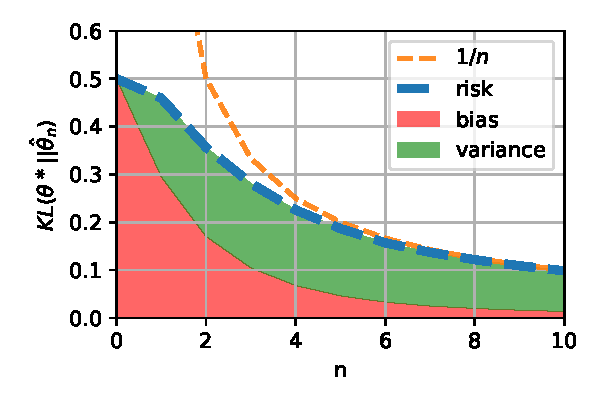
\includegraphics[width=.4\textwidth]{{figs/gaussians/new_linear_n0=1}.pdf}
	\caption{
	\textbf{Full gaussian} $\cN(m, \sigma^2)$ with $\meanp^*=(0, 1), \meanp_0 = (1,2)$ and $n_0=1$. \textbf{Left:} training curves (5,95) percentiles, average and asymptote.
	\textbf{Right:} bias-variance decomposition.
	}
	\label{fig:gaussian_decomposition}
\end{figure}


\section{Examples}


\subsection{Gaussian Variance}
A core example of this paper is a centered gaussian with unknown variance $\cN(0,\sigma^2)$.
The density is	$p(x) = \inv{\sqrt{2\pi \sigma^2}} e^{-\frac{x^2}{2 \sigma^2}}$.
Defining $T(X)=X^2$ as the sufficient statistic, we get natural parameter $\nat = -\inv{2 \sigma^2} <0$, and mean parameter $\m=\E[T(X)] = \sigma^2 >0$.
Mean and natural parameters are roughly inverse of each other $\nat = -\inv{2 \m}$.
Now we can match the log-likelihood with the exponential family template to get the log-partition function, and taking the conjugate to find the entropy
\begin{align}
	\logpart (\nat) &= - \half \log(-\nat)  + \half \log(\pi) \\
	\conj(\m) &= \half\left( -\log(\m) + \log\frac{\pi}{2} - 1 \right) \; .
\end{align}
Both the log-partition and  the entropy are roughly negative logarithm $z\mapsto - \log(z)$.
It means the conjugate prior is the exponential family with sufficient statistic $(\nat, \log(-\nat) )$, eg a negative Gamma distribution.
It also means $\bregman$ and $\bregmanconj$ have the same shape
\begin{align}
	\bregmanconj( \m_*; \m_n)
	&= \half \left ( \frac{\m_*}{ \m_n} - 1 - \log  \frac{\m_*}{ \m_n} \right) \\
	\bregman( \nat_n; \nat_* )
	&=  \half \left ( \frac{ \nat_n}{\nat_*} - 1 - \log  \frac{ \nat_n}{\nat_*} \right) \; .
\end{align}
In other words, this divergence measures the discrepancy between the ratio $\frac{ \nat_n}{\nat_*} =  \frac{\m_*}{ \m_n}  $ and $1$ via the function $\phi$
\begin{align}
	\phi(z) := \half (z - 1 - \log(z))
\end{align}
illustrated in Figure~\ref{fig:phi}.
Below we report upper bounds on the expected value of this divergence for the MLE and the MAP.


\begin{figure}[ht]
	\centering
	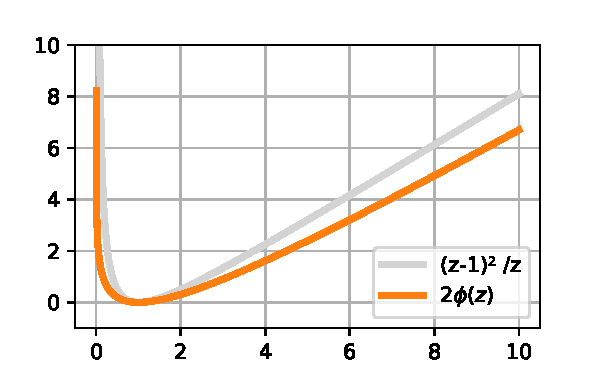
\includegraphics[width=.4\textwidth]{phi.pdf}
	\caption{$\phi(z)$ is the Bregman divergence induced by $-\log(z)$. It is a barrier near $0$. As a result, it is poorly approximated by quadratics, but it admits another upper-bound (in grey).}
	\label{fig:phi}
\end{figure}


\begin{theorem}[MLE Tight Bound]
	The MLE of $\cN(0,\m_*)$ is $\hat \m_n^\text{MLE} = \inv{n} \sum_i X_i^2 $.
	Its expected suboptimality is infinite when $n\leq 2$, and otherwise upper-bounded as
	\begin{align}
		 \expect{\bregmanconj( \m_*; \hat \m_n^\text{MLE}) }
			\leq \inv{2n} +\frac{2}{n(n-2)} \; .
			\label{eq:MLE_rate}
	\end{align}
\end{theorem}

This upper bound is asymptotically tight.
We illustrate its numerical behavior in Figure~\ref{fig:curves}.
We get a similar bound for the multivariate generalization :
the expected value is infinite whenever $n \leq d+1$ where $d$ is the dimension, and is otherwise bounded by $O(\frac{d^2}{n} + \frac{d^3}{n(n-d-1)} )$.

For the MAP, we get an upper bound thanks to the inequality $ - \log(z) \leq \inv{z} - 1$ which implies
\begin{align}
	\label{eq:log_bound}
	\phi(z) \leq \half (z + \inv{z}) - 1 = \frac{(z-1)^2}{2 z} \; .
\end{align}

\begin{theorem}[MAP Bound]
 For $n\in \naturalnumbers$, let us  define
 \begin{align}
	b_n = \frac{(1 + \inv{n_0} - \frac{\m_0}{\m^*})^2}{2 (\frac{\m_0}{\m^*}+\frac{(n-2)_+}{n_0})(1 + \frac{n}{n_0} )} \; .
 \end{align}
The expected suboptimality of the MAP of $\cN(0,\m^*)$ with prior hyper-parameters $(n_0,\m_0)$ is
 \begin{equation}
	\expect{\bregmanconj( \m_*; \hat \m_n^\mathrm{MAP})}
	\leq \begin{cases}
		\inv{2(n_0+1)}  +  b_1 \ \text{if}\ n=1,\\
		\frac{1}{n_0 \frac{\m_0}{\m^*} +n-2} + b_n \ \text{if}\ n\geq 2
	\end{cases}
	\label{eq:MAP_rate}
\end{equation}
\end{theorem}

This inequality highlights a clear variance-bias decomposition.
In particular, there is no bias term when $\frac{\m_0}{\m^*} =1 + \inv{n_0} $, which happens when the prior is slightly larger than the ground truth.  For instance, when $n_0=1$, it encourages us to set $\m_0 = 2 \m^*$. This correlates well with numerical observations.
Remark that the variance term is not asymptotically tight as the log-inequality we used \eqref{eq:log_bound} is not quadratically tight around $1$. We are basically losing a factor 2 compared to $1/2n$.


\begin{figure*}[t]
	\centering
	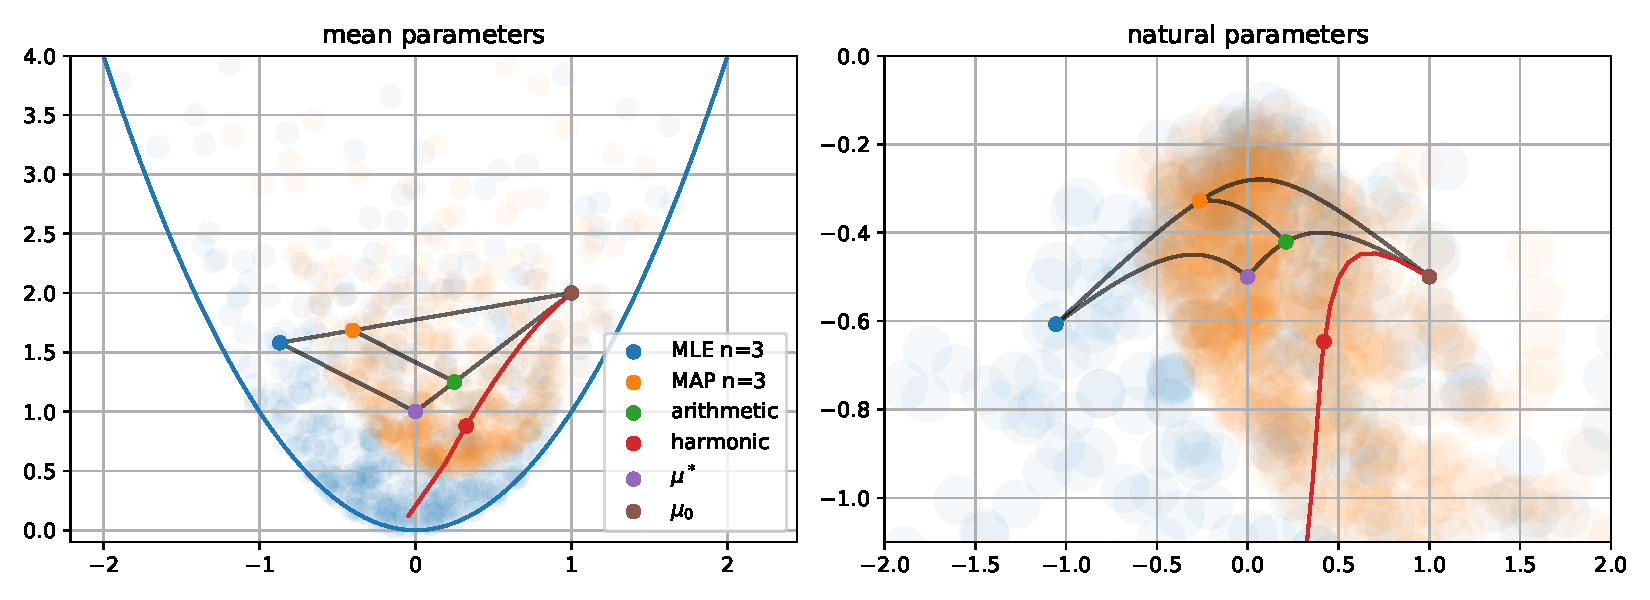
\includegraphics[width=\textwidth]{figs/thales/numerical_schema_n=3.pdf}
	\caption{A numerical illustration of the different characters featured in the bias-variance decomposition, for a 1D Gaussian $\cN(\mu, \sigma^2)$.}
	\label{fig:bias-variance-numerical}
\end{figure*}


\section{Optimization Perspective}
\label{sec:optimization}

We now show how MAP can be interpreted as stochastic mirror descent (SMD).
This means that 1. we may obtain a convergence rate for MAP from an optimization analysis, and 2. any insights gained from the MAP may inform further design and analysis of SMD.
We then review the assumptions of relative smoothness, useful to deal with non-smooth functions, before investigating 3 analysis of SMD with the MAP.
\rlp{mention that examples have so far been lacking for relative SMD.}

\subsection{MAP as Stochastic Mirror Descent}
\label{ssec:MAP=SMD}
By Bayes rule, the posterior can always be written iteratively $p(\nat | \mD_n) \propto p(X_n | \nat) p(\nat | \mD_{n-1})$.
Plugging in~\eqref{eq:joint_likelihood}, and introducing $f_n(\nat) = - \log p(X_{n} | \nat)$, we see that the MAP verifies
\begin{align*}
	\hat \nat_{n}
	= \argmin_\nat f_n(\nat) + (n_0 + n -1) \bregman(\nat; \hat \nat_{n-1})
    %\label{eq:SBPP}
\end{align*}
which is the update of a Stochastic Bregman Proximal Point update with step-size $\inv{n_0 + n - 1}$.
%Maybe skip this SBPP story altogether
Expanding $f_n(\nat) = \logpart(\nat) - T_n$ and  playing with the Bregman we get
\begin{align*}
		\hat \nat_{n}
	= \argmin_\nat \langle g_{n}(\hat \nat_{n-1}), \nat \rangle + (n_0 + n) \bregman(\nat; \hat \nat_{n-1})
    %\label{eq:SMD}
\end{align*}
where $g_{n}(\nat) := \nabla f_n(\nat) = \hat \m_{n-1} - T_n$.
We recognize the update of Stochastic Mirror Descent (a.k.a. Stochastic Bregman Gradient) with step-size $\lr_n = \inv{n_0 + n}$.
From the first order optimality condition, we see this is a stochastic gradient step in the dual $\hat \m_n = \hat \m_{n-1} - \lr_n g_n$.
This parallel means we could obtain a finite convergence rate for the  MAP from an analysis of these algorithms.
In particular, it could potentially apply to a wide range of distribution $\cD$ on $X$.
Note that this optimization perspective does not hold for the MLE %($n_0=0$)
as its implicit uniform prior may correspond to an initialization outside of $\Theta$.

\subsection{Relative Smoothness}
Mirror descent (MD)\footnote{
Also known as
Bregman (proximal) gradient, relative gradient descent or NoLips.
}
\citep{nemirovski1983problem,beck2003mirror}
%Nemirovski introduced the algorithm, and Beck established the connection with Bregman divergences, e.g. the argmin form.
and SMD 
\citep{nemirovski2009robust,ghadimi2012optimal} 
are typically encountered in non-smooth (online) optimization,
under bounded (or Lipschitz) gradient assumption on the objective $f$
and strong convexity assumption on the potential $\logpart$
\citep[Th.4.2 \& Th.6.3]{bubeck2015convex}.
In our case, none of these assumptions may hold. 
For instance $\logpart = -\log$ is neither smooth nor strongly convex.

\fdk{
{\bf Online learning paragraph?}
\citet{azoury2001relative,freund1996predicting,dasgupta2007online},
Bubeck's 2011.
}


Recently, these assumptions have been relaxed to allow for non-smooth functions $f$
\footnote{$f$ is $L$-smooth if its gradient is $L$-Lipschitz}.
and non-strongly convex potential $\logpart$, first in the deterministic setting
\citep{birnbaum2011distributed, bauschke2017descent, lu2018relatively}, then in the stochastic setting \citep{hanzely2018fastest, dragomir2021fast, dorazio2021stochastic}.
These assumptions have been replaced with
the $\mu$-strong convexity and $L$-smoothness of $f$
\emph{relative} to $\logpart$, defined as
\aligns{
	\mu \cB_{A}(x, y)
	\leq
	\cB_f(x,y)
	\leq
	L \cB_A(x,y) \; .
}
When $\logpart = \norm{\cdot}^2$, we recover standard (Euclidean) smoothness, and gradient descent. 
Those conditions ensure the linear convergence rate of MD with $A$ as the reference function.
Exponential families log-likelihood perfectly fit into this framework, as
\aligns{
	f(\theta) = A(\theta) - \expect{\lin{X, \theta}}
}
is $1$-smooth and $1$-strongly convex relative to $A$.

\subsection{Bounding the Randomness}
Smoothness is not the only issue.
To analyze stochastic algorithms, one also need to quantify the randomness.
Many assumptions exist for SGD \citep[\S3 for a modern review]{khaled2020better}.
We now review attempts at analyzing SMD under relative smoothness assumption, in the light of  the MAP example.
See \cref{tbl:assumptions} for a summary.

Caveat : all of these rates apply to the Bregman in the other direction, e.g. $\bregman(\nat^*, \MAPt)$, and sometimes not on the last iterate, but with tail averaging.

\begin{table}[t]
\begingroup
\renewcommand*{\arraystretch}{1.25}%
\newcommand*{\greencmark}{\textcolor{Green}{\cmark}}
\newcommand*{\redxmark}{\textcolor{Red}{\xmark}}
\centering
\begin{tabular}{lccc}
%{p{.15\textwidth}m{.05\textwidth}m{.08\textwidth}m{.1\textwidth}}
\toprule
Boundedness & Barriers &  $\lr_n \sim \inv{n}$ & Last iterate \\
\midrule
%Strongly convex and bounded variance\newline
%\citep[e.g.,][]{??}
%&
%$
%\cB_A(\theta,\theta') \geq \frac{1}{2}\norm{\theta-\theta'}^2,
%\quad
%\expect[x]{\norm{\m - x}}^2\leq\sigma^2
%$
%\\
Variance $\forall \nat\in\Theta$~\eqref{eq:hanzely} % \newline \citep{hanzely2018fastest}
& \redxmark & \greencmark  & \redxmark
\\
Variance at $\theta_*$~\eqref{eq:dragomir} %\newline \citep{dragomir2021fast}
& \redxmark & \greencmark  & \greencmark
\\
Optimality gap~\eqref{eq:dorazio} %\newline \citep{dorazio2021stochastic}
& \greencmark & \redxmark & \greencmark
\\
\bottomrule
\end{tabular}
\caption{
Summary of results about SMD with relative smoothness and relative strong convexity assumptions. 
Barrier tells whether the assumption can hold with barrier objectives.
$\lr_n \sim \inv{n}$ says whether the convergence rate hold with this step-size scheduling, and the last column tells whether the rate applies to the last iterate or to some average iterate.
}
\label{tbl:assumptions}
\endgroup
\end{table}

\subsubsection{Bounded Variance}
\citet{hanzely2018fastest} assume the covariance between negative gradient and next iterate is upper bounded at every time step: $\forall n \geq 1, \forall \hat \nat_{n-1},$
\alignn{
\Cov(-g_n(\hat \nat_{n-1}) , \MAPt) \leq \lr_n C
\label{eq:hanzely}
}
for some constant $C$.
For a Gaussian with known variance ($A(\theta) = \frac{1}{2}\norm{\theta}^2$),
this definition recovers the variance of the stochastic gradient
$\expect[\tilde g_t\!\!]{\norm{\nabla f(\theta) - \tilde g(\theta)}{}^2}\leq C$.
More generally, if $A$ is $\mu$-strongly convex in $\norm{\cdot}$,
the LHS of \cref{eq:hanzely} is bounded by
$\expecti{\frac{1}{\mu}\norm{\nabla f(\theta) - \tilde g(\theta)}{}^2_*}$,
and a bound on the variance of the stochastic gradient is a sufficient condition for \cref{eq:hanzely}
to hold.
Another perspective on this covariance is as the expectation of the symmetrized Bregman $\cS_\conj(\m_1, \m_2) = \bregmanconj(\m_1, \m_2) + \bregmanconj(\m_2, \m_1)$ between stochastic and deterministic updates
\aligns{
\Cov(-g_n(\hat \nat_{n-1}) , \MAPt) = \E[\cS(\MAPm - \lr g_n  )]
}
thus showing positivity.
Under this assumption, they prove a $O(1/n)$ convergence rate with a $O(1/n)$ step-size \citep[Lem.4.8]{hanzely2018fastest}, by applying a polynomial tail averaging \citep{lacostejulien2012simpler} in primal space $\Theta$.

In general however, this assumption hardly holds.
For the MAP, this translates into $\forall n \geq 1,$
\alignn{
\expect[T_n]{\lin{T_n - \mu^* , \MAPt}} \leq \lr_n C
}
which fails to hold on the gaussian variance example for instance. \TODO{short proof or formalize.}

\subsubsection{Bounded Variance at the Minimum}

\citet{dragomir2021fast} introduce a much weaker assumption $\forall n \geq 1, \forall \MAPm,$
\alignn{
	\expect[\tilde g]{
		\cB_{A^*}(\MAPm - 2\lr g(\theta_*), \MAPm)
	} \leq 2 \lr^2 C \; .
	\label{eq:dragomir}
}
In words, this is bounding the variance of the gradients at the minimum, but with a metric that depends on the iterate $\MAPm$, and this bound should hold for every iterate we may encounter on the stochastic trajectory.
% As observed by Frederick, this is really weaker than Hanzely, because it is only the first half of their assumption. There is only a factor 2 that's preventing a direct inequality. 
Under this assumption, they prove convergence up to a variance ball with a constant step-size.
Their descent lemma \citep[Eq.(12)]{dragomir2021fast} is the exact analog  of a modern analysis of SGD \citep[Th.3.2]{gower2019sgd}, meaning we can plug in a $O(1/n)$ decreasing step-size and obtain a $O(1/n)$ convergence rate.

Seems like a perfect fit then ? Well not really, this variance assumption does not hold for exactly the same reason as the one of Hanzely. Having something valid for every possible iterates is way too strong. 

\subsubsection{Bounded Optimality Gap}
Inspired by \citet{loizou2021stochastic}, \citet{dorazio2021stochastic} explores the hypothesis
\alignn{
\min_\nat f(\nat) - \expect[X]{\min_\nat f_X(\nat)} \leq C 
\label{eq:dorazio}
}
where $f_X$ is a stochastic estimate of $f = \expecti{f_X}$. In our case $f_X(\nat) = - \log p(X\cond \nat)$.
In words, this is lower bounding the expectation of the minimum of these stochastic estimates.
For probabilistic models, such a bound is finite as soon as the model cannot give infinite density to any data point $x$.
This holds for instance for discrete distributions 
-- $f_x\geq 0$ because the probability mass is upper bounded by $1$ -- 
but it rules out  many families.
For normal distributions set $\mu=x$ and $\sigma^2 \rightarrow 0$ to get $p(x\cond \nat) \rightarrow +\infty$. 
For gamma, set $\alpha = \beta x$ and $beta \rightarrow +\infty$.
For beta, set $\alpha=\beta \frac{x}{1-x}$ and $\beta \rightarrow +\infty$.
 Other examples include inverse Gaussians, log-normal, gamma, inverse gamma.
 
 It is possible to overcome this limitation though, by treating batches of samples as 1 sample, and averaging sufficient statistics -- e.g. $Y = \{X_1, \dots, X_k\}$ and $T(Y) = \inv{k}\sum_i T(X_i)$.
 For instance a multivariate normals of dimension $d$ cannot attribute infinite density to $d+1$ samples that are not in an affine subspace.

So it seems this approach can yield interesting convergence rates for the MAP, and they do prove linear convergence of the last iterate up a to a variance ball with constant step-size, but the size of this ball $\frac{C}{\alpha}$ \rlp{strong convexity notation} is independent of  the step-size. Their descent lemma does not lead to convergence with a decreasing $O(1/t)$ step-size. 


\subsection{Issues with current analyses}

\fdk{They don't hold for problems we care about}

\fdk{Existing techniques only deal with fixed step-sizes and show convergence to a ball}

If assumptions~\eqref{eq:hanzely} and~\eqref{eq:dragomir} do not hold for every iterate, then let's assume they hold on average. Does the proof remain valid ? Yes I think so \TODO{check this}. Does it become impossible to prove / as hard as the initial problem ? Yes.
\TODO{Does it match exactly the variance from the bias-(mixed)-variance decomposition ?}

\section{Conclusion}
Exponential family MLE and MAP are used everywhere -- everytime someone computes a mean and variance to fit some bell-shaped data. 
MLE and MAP are both maximizing the (regularized) likelihood of the data, whose suboptimality is the Kullback-Leibler (KL) divergence.
The KL is a very natural measure of discrepancy between a model and the true disribution.
Yet we do not have convergence rates on the expected KL, even in the well-specified setting.
Such a rate could inform us on how many samples we may need, or on the influence of the prior.
There are many results close from such a rate, in particular large sample results \citep{kakade2010learning, ostrovskii2021finite}, which describe how many samples are needed to ensure a locally quadratic regime.
Another approach to obtain rates is stochastic optimization \citep{bach2013nonstronglyconvex}. 
Here we observed that MAP perfectly fits the framework of stochastic mirror descent with relative smoothness assumptions.
Yet none of the current analysis of SMD hold for the MAP, even on a simple family such as $\cN(0,\sigma^2)$, thus revealing area for progress in non-Euclidean optimization.
In writing this paper, we hope to attract attention to this fundamental problem, leading to progress in both optimization and statistics.



\newpage
\bibliographystyle{apalike}
\bibliography{references.bib}


\clearpage
\section{Group Meeting}
\begin{enumerate}
	\item new plots : mirror map, and gaussian trajectories. Add trajectories to paper, with background level set, and new legend : primal/dual expectation
	\item the MLE is biased according to our definition. See plots. Does this definition of bias make sense ? An unbiased estimator's primal mean would be equal to the optimum, vs the dual mean.  Remark : the MLE is biased for standard parameters.
	\item exciting pap er\citet{kakade2010learning}
	\begin{enumerate}
		\item assumption in the spirit of infinite order self-concordance only at the optimum
		\item After a burn-in phase, the loss behaves quadratically. No precise description of the burn-in length.
		\item \TODO{it is worth writing down until the end what we are obtaining with self-concordance.}
		\item idea 1 : try to express some of their results with the mean parameter instead.
		\item idea 2 : using their assumption on the mirror map, perform a Newton kind of analysis for SMD. (exploiting the link MAP -> optimization). How do we prove the linear convergence of Newton to the quadratic regime ? That is the problem at stake here.
	\end{enumerate}
	\item Intro : positioning between optimization and statistics. Start with stats. Convince the reader that this is an essential problem, with asymptotic rate. but finite is elusive. Inspired by recent work (lepriol2021 , bach2013) we want to use optimization to give a rate. We fail, but we reveal a hole in current analysis.  Finite rate would allow us to quantify the importance of the prior, and also help us understand behavior for small numbers.
	\item Intro : 1 clear question and sharper contributions, with references to sections, as a memo for the reviewer writing his review. "investigate bias-variance..." "we show all these analysis suffer from this problem."
	\item Organization : add optim parallel in insigths section, and then sprinkle references until the optim section.
	\item Optim : find members of the exponential family where the rate of Dragomir et al. holds.
	\item Technical Background : be precise and add reference for the steep exponential family of Legendre type which guarantees that our sets are open, and have a solution in the middle.
	References: \begin{itemize}
		\item \href{https://www.jstor.org/stable/4616462?seq=1#metadata_info_tab_contents}{Existence of Maximum Likelihood Estimates for Multi-Dimensional Exponential Families},
		\item The singly truncated normal distribution: A non-steep exponential family,
		\item Statistical exponential families: A digest with flash cards,
		\item Information and Exponential Families In Statistical Theory,
		\item Fundamentals of Statistical Exponential Families with Applications in Statistical Decision Theory.
	\end{itemize}
\end{enumerate}




\section{Blurbs/ideas?}



\subsection{SGD blurb}
\fdk{
%
There is a long line work bounding the convergence rate of stochastic gradient descent.
Beyond the results of \citet{robbins1951stochastic},
we now have proofs on smooth, strongly convex problems and bounded variance
(as well as other assumptions on the noise, reviewed later)
a decreasing step-size and an averaging scheme gets
a $1/t$ convergence rate,
which matches the asymptotic rate of unbiased estimation,
through clever averaging schemes \citep{rakhlin2012making,lacostejulien2012simpler}
\\
Those papers assume the stochastic gradients are bounded,
but small modifications also work for bounded variance instead.
\\
We do have extensions to other notions of bounded variance,
for example assuming that the stochastic gradients are gradients of a perturbed smooth function $f_i$
and that the minimum of $f$ and the minima of the $f_i$
are bounded, $\expect{\min_x f(x) - \min_x f_i(x)} \leq \sigma^2$,
or that the gradient noise is bounded only at the minimum.
For a review, see \citet{gower2019sgd}.
\\
However, for some problems, combining decreasing step-sizes and averaging is not necessary,
even when the function is not strongly convex.
This is the case for maximum likelihood estimation and matches the asymptotic rates,
but holds more generally, for example for linear and logistic regressions \citep{bach2013nonstronglyconvex,moulines2011non}.
}


\subsection{Poisson likelihood?}
\fdk{
\citet{bauschke2017descent} and \citet{hanzely2018fastest} both use the example of Poisson inverse problems/Poisson regression
as examples.
The simpler case of the MLE of a Poisson distribution is also unsolved, though.
In this case, $h(x) = 1/x!$, $x \in \mathbb{N}$, $A(\theta) = e^\theta$ over $\theta \in \mathbb{R}$,
$A^*(\m) = \m \log \m - \m$ over $\m \in \mathbb{R}_+$.
It is neither strongly-convex nor self-concordant (at least according to the standard definition,
although it satisfies generalized notions of self-concordance as $A'''(\theta) = A''(\theta)$).
}

\subsection{``simple'' open problem?}
\fdk{
A ``simple open problem'';
assume we have a deterministic problem, so that we know where the minimum is.
Can we figure out a (deterministic) path from $\theta_0$ to $\theta_*$
that has optimality decreasing as $1/n^2$,
to mirror the bias term of gradient descent?
}

\subsection{Connection with acceleration?}
\fdk{
The problems on how to deal with Bregman divergences abound in optimization, beyond stochasticity.
For example, we haven't yet figured out the analog of Nesterov-type acceleration
on relatively smooth and strongly convex problems,
to bring the convergence rate from linear in $(1-\kappa)$ to $(1-\sqrt{\kappa})$,
or just from $1/T$ to $1/T^2$ in the (non-strongly) convex case.
\citet{dragomir2021optimal}  shows that naïve application of Bregman updates can not achieve acceleration.
The tools developed to make progress on one problem might help make progress on the other.
}










\newpage
\section{Notation convention}
We use
\begin{itemize}
	\item $\theta, \nat$ for natural parameters
	\item $\m$ for mean parameters
	\item $X_1,\ldots,X_n$ for data
	\item $\cX$ for the data space
	\item $T$ for the sufficient statistics
	\item $\nu$ for the base measure
	\item $A, A^*, \logpart, \conj$ for the log-partition and its dual
	\item $\cB_A$ for the Bregman divergence induced by $A$
	\item $n$ for the number of samples
	\item $(\theta^*,m^*)$ for the optimum
	\item $\gamma, \lr$ for the step-size
	\item $\mu,\sigma^2$ for the parameters of a Gaussian
	\item $\hat\theta_n$ for estimates
	\item $\tilde\theta_n$ for $\expect{\hat\theta_n}$, which is biased
	\item $(L, \mu)$ for strong-convexity and smoothness
\end{itemize}

\fdk{
	Do we use $\alpha, \beta$ anywhere?
	Might use those for smoothness/strong-convexity rather than $\mu, L$.
}

\fdk{
	The superscript ${}^*$ denotes the convex conjugate when applied on a function
	and the optimum when applied to a parameter.
	How about we use $\theta_n, \theta_*$ for parameter at time $n$ and at the optimum
	and $f^*$ for the convex conjugate?
}

\fdk{
	On $X_i$ for data; I'm more used to seeing $x_i$ for data, which is the realization of the random variable $X_i$.
	We don't talk about random variables and don't need the distinction?
}

\fdk{
	Need to check
}

\end{document}